\documentclass[10pt,pdf,hyperref={unicode}]{beamer}
\beamertemplatenavigationsymbolsempty
\setbeamertemplate{footline}[page number]

\usepackage[utf8]{inputenc}
\usepackage{bm}
\usepackage{multirow}
\usepackage{ragged2e}
\usepackage{indentfirst}
\usepackage{multicol}
\usepackage{subfig}
\usepackage{amsmath,amssymb}
\usepackage{enumerate}
\usepackage{mathtools}
\usepackage{tikz}
\usetikzlibrary{positioning,arrows}
\usepackage{pgfplots}
\pgfplotsset{compat=1.18}
\definecolor{graycolor}{rgb}{0.5,0.5,0.5}

% Colors
\definecolor{darkgreen}{rgb}{0.0, 0.2, 0.13}
\definecolor{darkcyan}{rgb}{0.0, 0.55, 0.55}

%----------------------------------------------------------------------------------------------------------

\title{Next Year's Cash-Flow Forecasting}
%\author{Name Surname}
%\institute[]{}
%\date{2024}

%----------------------------------------------------------------------------------------------------------

\begin{document}
	
	\setcounter{page}{1}
	
	% First slide: Overview of the problem and solution
	\begin{frame}{Next Year's Cash-Flow Forecasting}
		
		\begin{block}{The Problem}
			Accurate cash flow forecasting is crucial for budgeting, managing liquidity, and identifying investment opportunities. The challenge is to develop a model that includes both internal financial metrics and external economic indicators (e.g., market 
			trends, inflation).
		\end{block}
		
		\begin{block}{The Solution}
			We will develop a forecasting model using advanced time series forecasting techniques:
			\begin{itemize}
				\item ARIMA for historical trend analysis,
				\item Prophet for seasonal components,
				\item LSTM for deep learning on sequential data.
			\end{itemize}
			This will provide the finance department with reliable forecasts for budget planning and liquidity management.
		\end{block}
		
	\end{frame}
	
	\setcounter{page}{2}
	
	% Second slide: Visual representation of the solution
	\begin{frame}{Illustrative Example: Forecasting Solution}
		
		\begin{columns}
			\begin{column}{0.35\textwidth}
				\begin{enumerate}
					\item Historical Data: 5 years of monthly cash flow data.
					\item External Factors: Market trends, inflation rates.
					\item Time Series Models: ARIMA, Prophet, LSTM.
				\end{enumerate}
			\end{column}
			
			\begin{column}{0.7\textwidth}
				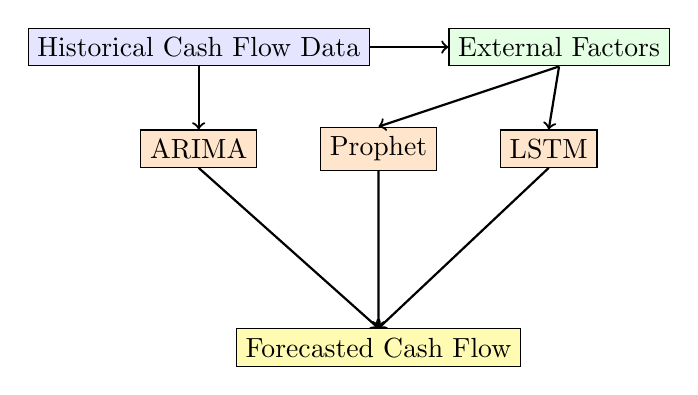
\begin{tikzpicture}[scale=0.9]
					% Drawing the time series forecasting process
					\node (data) [rectangle, draw, fill=blue!10] {Historical Cash Flow Data};
					\node (factors) [rectangle, right=of data, draw, fill=green!10] {External Factors};
					
					\path[->] (data.east) edge [thick] (factors.west);
					
					\node (arima) [rectangle, below=0.8cm of data, draw, fill=orange!20] {ARIMA};
					\node (prophet) [rectangle, right=0.8cm of arima, draw, fill=orange!20] {Prophet};
					\node (lstm) [rectangle, right=0.8cm of prophet, draw, fill=orange!20] {LSTM};
					
					% Connecting the models to the final forecast
					\path[->] (data.south) edge [thick] (arima.north);
					\path[->] (factors.south) edge [thick] (prophet.north);
					\path[->] (factors.south) edge [thick] (lstm.north);
					
					\node (forecast) [rectangle, below=2cm of prophet, draw, fill=yellow!30] {Forecasted Cash Flow};
					\path[->] (arima.south) edge [thick] (forecast.north);
					\path[->] (prophet.south) edge [thick] (forecast.north);
					\path[->] (lstm.south) edge [thick] (forecast.north);
				\end{tikzpicture}
			\end{column}
		\end{columns}
		
	\end{frame}
	
\end{document}
